\chapter{Proposed Translator}
\label{ch:proposed-system}
As a solution to the previous chapter, this one focuses on proposing a application $f : SC' \rightarrow MO$ such that applied on a
schema, defined in \cref{eq:schema-reduction}, results in a domain model (\cref{eq:plain-object-model}) based on plain objects (\cref{eq:plain-object}).
Therefore the aim of this chapter is to once defined an schema as \cref{eq:schema-reduction} and a shape as \cref{eq:shape-reduction} define
an application $f$ such that

\begin{equation}
f(SC')=
\begin{bmatrix}f'(S'_1)
\\ f'(S'_2)
\\ \vdots
\\ f'(S'_n)
\end{bmatrix},
\end{equation}

where,

\begin{equation}
	f'(p_{SC'},t_{SC'},c_{SC'}) = (p_{S'},t_{S'}),
\end{equation}

and give a proposition for $f'(x')$ and therefore for $f(x)$.

We know that \cref{eq:shape-reduction} has been obtained in such a way that $\forall\ s' \in S'\ \exists\ f:S' \rightarrow PO$ and also in \cref{eq:values-mapping} we set
the aggregation criterion of the cardinality component over the type component to be able to create the images of $SC'$ in $MO$. Therefore $f'$ is defined as,

\begin{equation}
f':S' \rightarrow PO = f(p_{S'},t_{S'},c_{S'}) \begin{cases}
	(p_{S'},\ Proy_{t_{S'}}lst) & if \; c_{S'}=(1,1) \\
	(p_{S'},\ List[Proy_{t_{S'}}lst]) & if \; c_{S'}=(0,\infty)
   \end{cases}.
\end{equation}

Therefore we not only know that it is possible to create a transformation from the subset of selected schemas
towards domain models formed by flat objects, but we have also identified the function that allows us to carry
out this transformation. So, next we will focus on giving shape to this function so that a system can be
implemented that performs the described transformations automatically.For this, in this section we will see
the structure of the proposed solution as well as an implementation that allows us to validate the proposed
solution to later analyze the objects generated by the solution.

\section{Structure}
At the very end a code translator is a kind of compiler where you should have a front-end, that
analyzes the input source code and checks that everything is correct, and a back-end that
generates the code in the target language. The main difference between generating code encoded
in a single language or in multiple languages is the number of specific translators that you will need to
implement, but all of them will be grouped in the bac-end. Therefore we will separate our
translator in \textbf{front-end} and \textbf{back-end}.

\subsection{Front-end}
The front-end task is to parse, analyze and validate the input source code. This might seem familiar to
\cref{ch:proposed-sintactic-semantic-analyzer} and it is in fack because in that chapter we define
a compiler front-end. Therefore we will re-use the same backend and we will continue to develope this
chapter from the \textit{Intermediate Language} that was generated at the end of the process described in
\cref{fig:shex-lite-sema}.

\subsection{Back-end}
The back-end of a translator, also known as the \textit{sinthesis} takes the previous \textit{Intermediate Language}
and translates it to the desired target language. \cref{fig:translation-function} illustrates this process.

\begin{figure}
    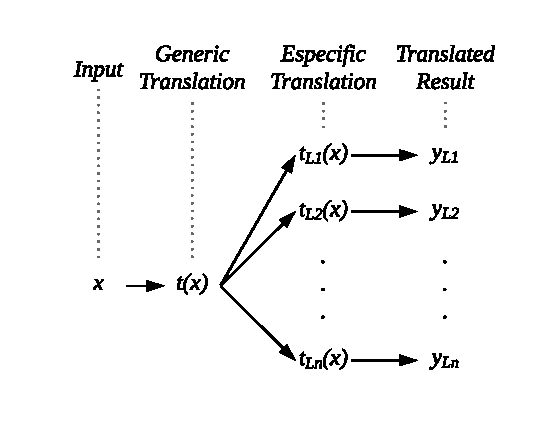
\includegraphics{images/translation-function.pdf}
    \centering
	\caption[Generic translation function structure]{Generic translation function structure for multiple
	target languages.}
    \label{fig:translation-function}
\end{figure}

\section{Implementation}

\section{Generated Obejcts}

\begin{figure}
    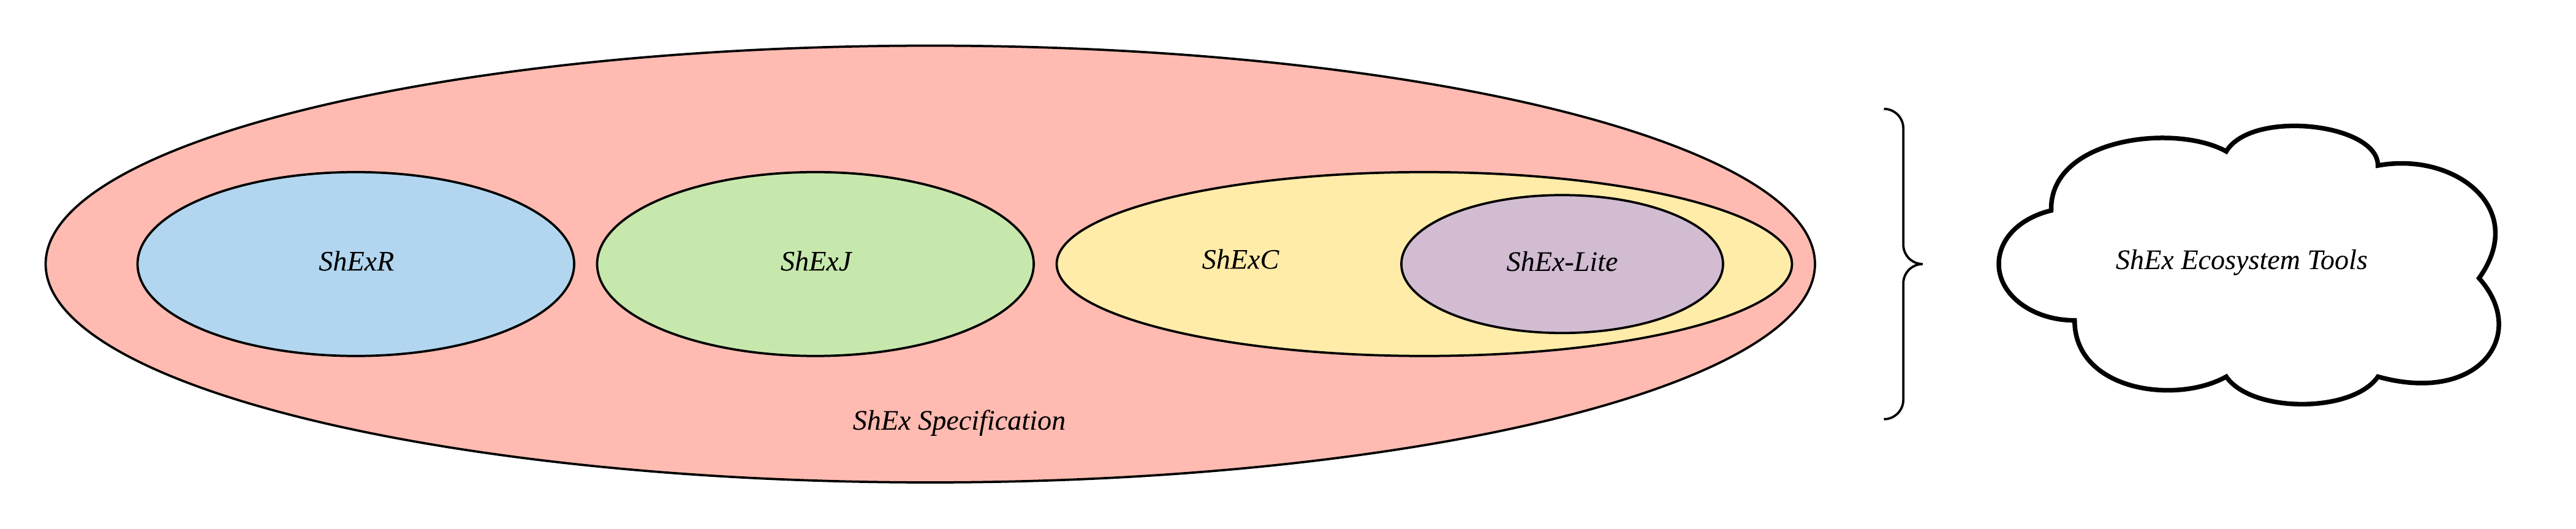
\includegraphics[width=\textwidth]{images/shex-lite-syntaxes-mental-model.png}
    \centering
    \caption[Mental model of ShEx-Lite in the existing ShEx syntaxes context.]{Mental model of
    ShEx-Lite in the existing ShEx syntaxes context. From this model we can see that Shex-Lite
    is in fact an strictly subset of ShExC, which follows the ShEx Specification. And therefore
    ShEx-Lite will also follow that expecification, which automatically enables ShEx-Lite schemas
    to be used in any other existing ShEx tool.}
    \label{fig:syntax-mental-model}
\end{figure}

\begin{figure}
  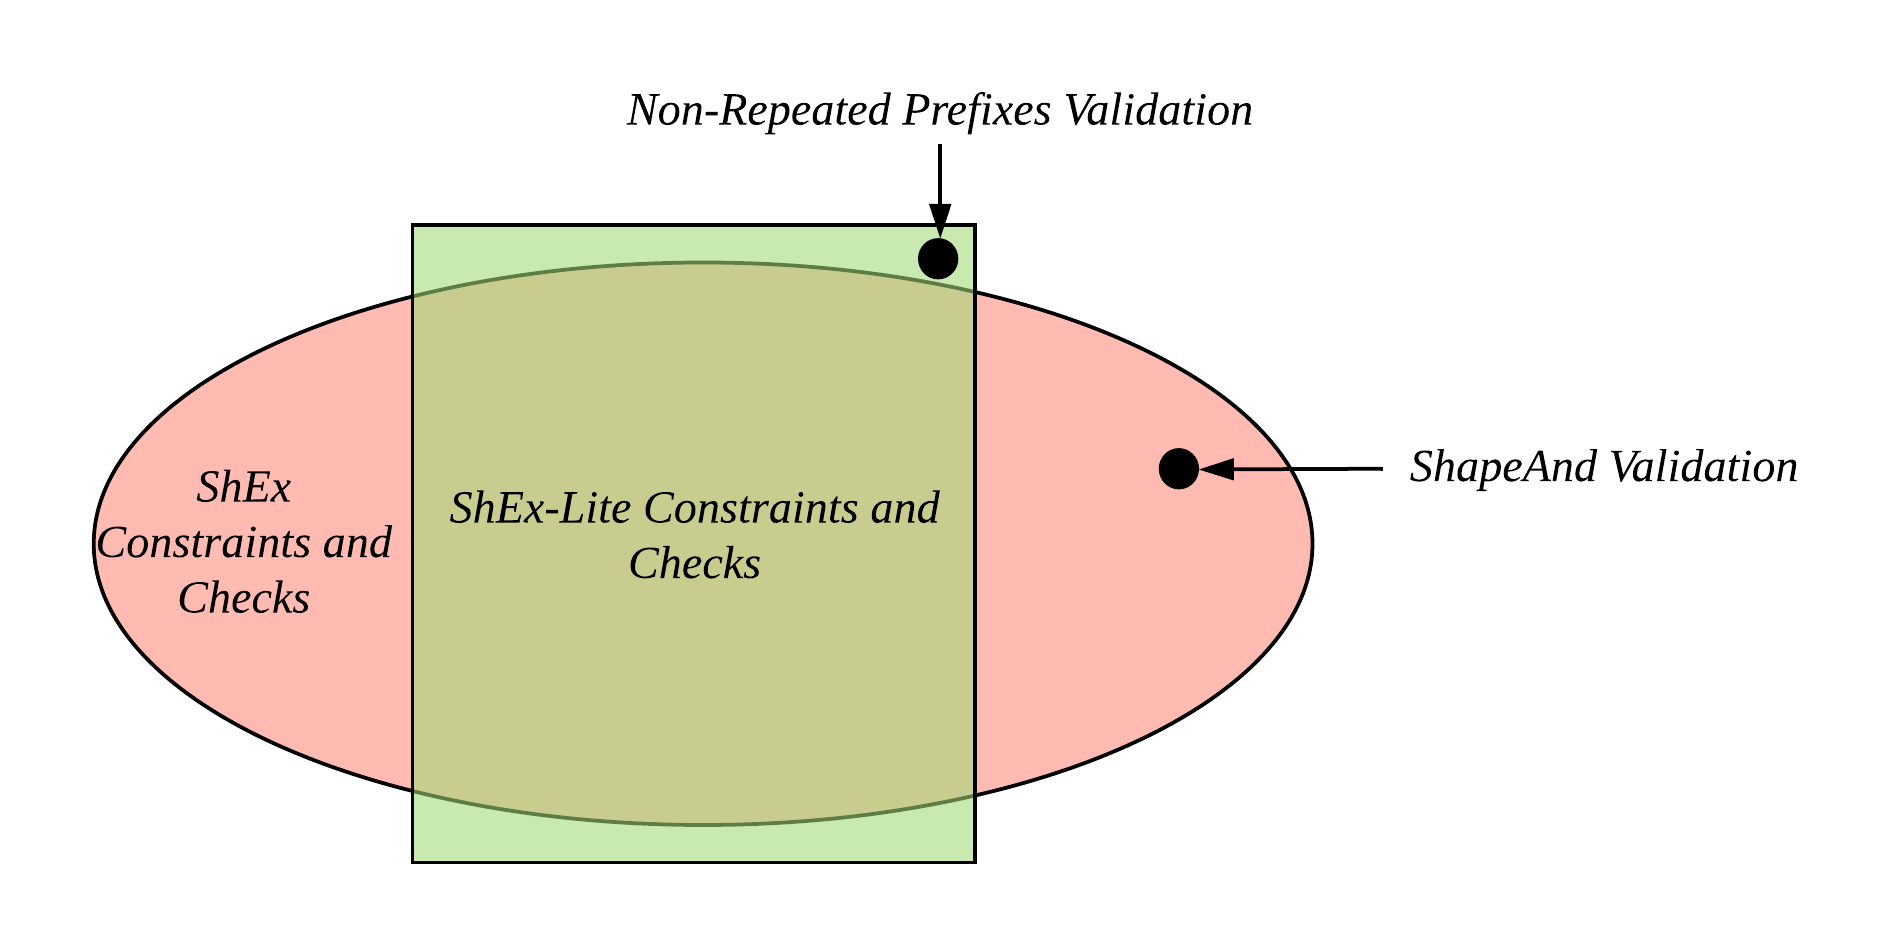
\includegraphics[width=\textwidth]{images/shex-lite-constraints-context.png}
  \centering
  \caption[Constraints and checks context diagram for ShEx-Lite and ShEx.]{Constraints
  and checks context diagram for ShEx-Lite and ShEx.}
  \label{fig:constraints-context}
\end{figure}

\begin{center}
	\noindent\begin{minipage}[t]{.4\textwidth}
		\begin{lstlisting}[frame=topline,numbers=left,title=\scriptsize\texttt{Person.shexl}, basicstyle=\ttfamily\scriptsize]{a}
# Prefixes...
:Person {
	:name xsd:string ;
	:knows @:Person *
}
		\end{lstlisting}
	\end{minipage}\hfill
	\begin{minipage}[t]{.5\textwidth}
		\begin{lstlisting}[language=Java, frame=t,numbers=left,title=\scriptsize\texttt{Person.java}, basicstyle=\ttfamily\scriptsize]{b}
// Imports...
public class Person {
	private String name;
	private List<Person> knows;
	// Constructor...
	// Getters and Setters...
}
		\end{lstlisting}
	\end{minipage}
	\captionof{figure}{Schema modeling a \texttt{Person} in \texttt{shexl} syntax to the left. And the \texttt{ShEx-Lite} generated code in \texttt{Java} to the right.}
	\label{fig:example-1}
\end{center}